\documentclass[11pt]{article}\usepackage[]{graphicx}\usepackage[]{color}
% maxwidth is the original width if it is less than linewidth
% otherwise use linewidth (to make sure the graphics do not exceed the margin)
\makeatletter
\def\maxwidth{ %
  \ifdim\Gin@nat@width>\linewidth
    \linewidth
  \else
    \Gin@nat@width
  \fi
}
\makeatother

\definecolor{fgcolor}{rgb}{0.345, 0.345, 0.345}
\newcommand{\hlnum}[1]{\textcolor[rgb]{0.686,0.059,0.569}{#1}}%
\newcommand{\hlstr}[1]{\textcolor[rgb]{0.192,0.494,0.8}{#1}}%
\newcommand{\hlcom}[1]{\textcolor[rgb]{0.678,0.584,0.686}{\textit{#1}}}%
\newcommand{\hlopt}[1]{\textcolor[rgb]{0,0,0}{#1}}%
\newcommand{\hlstd}[1]{\textcolor[rgb]{0.345,0.345,0.345}{#1}}%
\newcommand{\hlkwa}[1]{\textcolor[rgb]{0.161,0.373,0.58}{\textbf{#1}}}%
\newcommand{\hlkwb}[1]{\textcolor[rgb]{0.69,0.353,0.396}{#1}}%
\newcommand{\hlkwc}[1]{\textcolor[rgb]{0.333,0.667,0.333}{#1}}%
\newcommand{\hlkwd}[1]{\textcolor[rgb]{0.737,0.353,0.396}{\textbf{#1}}}%
\let\hlipl\hlkwb

\usepackage{framed}
\makeatletter
\newenvironment{kframe}{%
 \def\at@end@of@kframe{}%
 \ifinner\ifhmode%
  \def\at@end@of@kframe{\end{minipage}}%
  \begin{minipage}{\columnwidth}%
 \fi\fi%
 \def\FrameCommand##1{\hskip\@totalleftmargin \hskip-\fboxsep
 \colorbox{shadecolor}{##1}\hskip-\fboxsep
     % There is no \\@totalrightmargin, so:
     \hskip-\linewidth \hskip-\@totalleftmargin \hskip\columnwidth}%
 \MakeFramed {\advance\hsize-\width
   \@totalleftmargin\z@ \linewidth\hsize
   \@setminipage}}%
 {\par\unskip\endMakeFramed%
 \at@end@of@kframe}
\makeatother

\definecolor{shadecolor}{rgb}{.97, .97, .97}
\definecolor{messagecolor}{rgb}{0, 0, 0}
\definecolor{warningcolor}{rgb}{1, 0, 1}
\definecolor{errorcolor}{rgb}{1, 0, 0}
\newenvironment{knitrout}{}{} % an empty environment to be redefined in TeX

\usepackage{alltt}
%\usepackage[showframe]{geometry}
\usepackage[table]{xcolor}
\usepackage{caption}
\usepackage{lscape,verbatim,mathrsfs}
\usepackage{graphics,amsmath,pstricks}
\usepackage{amssymb,enumerate}
\usepackage{amsbsy,amsmath,amsthm,amsfonts, amssymb}
\usepackage{graphicx, rotate, array}
\usepackage{geometry,multirow}
\usepackage{color,soul}
\usepackage{float}
%\usepackage{hyperref}
\usepackage[authoryear,round]{natbib}
%\renewcommand{\baselinestretch}{1.9}
\usepackage{tcolorbox}
\renewcommand{\familydefault}{cmss}
\textwidth=6.65in \textheight=9.7in
\parskip=.025in
\parindent=0in
\oddsidemargin=-0.1in \evensidemargin=-.1in \headheight=-.6in
\footskip=0.5in \DeclareMathOperator*{\argmax}{argmax}
\DeclareMathOperator*{\argmin}{argmin}
\IfFileExists{upquote.sty}{\usepackage{upquote}}{}
\begin{document}

The purpose of this simulation study is to examine different ways of evaluating an ODTR. Specifically, we examine how different estimators (unadjusted, g-comp, IPTW, IPTW-DR, TMLE, CV-TMLE) do with approximating the statistical parameter $E_0[Y_{d_0}]$ and the data-adaptive parameter $E_0[Y_{d_n}]$, under different SL ODTR estimators (ie different SL libraries, varying in ``aggressiveness"). Here, $d_0$ is true optimal rule, $d_n$ is estimate of optimal rule.










\section{Description of DGP}

\begin{align*}
W_1,W_2,W_3,W_4 &\sim Normal(\mu=0,\sigma^2=1) \\
A &\sim Bernoulli(p=0.5) \\
Y &\sim Bernoulli(p) \text{ .}\\
\end{align*}
\begin{align*}
p &= 0.5*logit^{-1} (1-W_1^2  + 3W_2  + 5W_3^2 A - 4.45A)+0.5logit^{-1} (-0.5- W_3  + 2W_1 W_2  + 3|W2|A - 1.5A) \text{ ,}
\end{align*}
True blip function is:
\begin{align*}
    B_0 (W)= & 0.5[logit^{-1} (1-W_1^2  + 3W_2  + 5W_3^2  - 4.45)+logit^{-1} (-0.5- W_3  + 2W_1 W_2  + 3|W2|  - 1.5)\\
& - logit^{-1} (1-W_1^2  + 3W_2 )+logit^{-1} (-0.5- W_3  + 2W_1 W_2 )] \text{ .}
\end{align*}







\section{Library legend}

\begin{itemize}
\item Incorrect GLM
\begin{itemize}
\item QAW.SL.library = linear model main terms W and A and interaction with W and A
\item blip.SL.library = linear model with main terms W
\end{itemize}
\item GLMs
\begin{itemize}
\item QAW.SL.library = linear model with $W_j$ and A as main terms and $W_j$*A interaction for each $j$
\item blip.SL.library = linear model with main terms $W_j$ for each $j$
\end{itemize}
\item ML + GLMs not aggressive
\begin{itemize}
\item QAW.SL.library = GLMs library AND SL.glm, SL.mean, SL.glm.interaction, SL.earth, SL.nnet, SL.svm, SL.rpart
\item blip.SL.library = GLMs library AND SL.glm, SL.mean, SL.glm.interaction, SL.earth, SL.nnet, SL.svm, SL.rpart
\end{itemize}
\item ML + GLMs not aggressive
\begin{itemize}
\item QAW.SL.library = ML + GLMs aggressive library AND SL.randomForest
\item blip.SL.library = ML + GLMs aggressive library AND SL.randomForest
\end{itemize}
\end{itemize}

\section{Results}
\begin{knitrout}
\definecolor{shadecolor}{rgb}{0.969, 0.969, 0.969}\color{fgcolor}
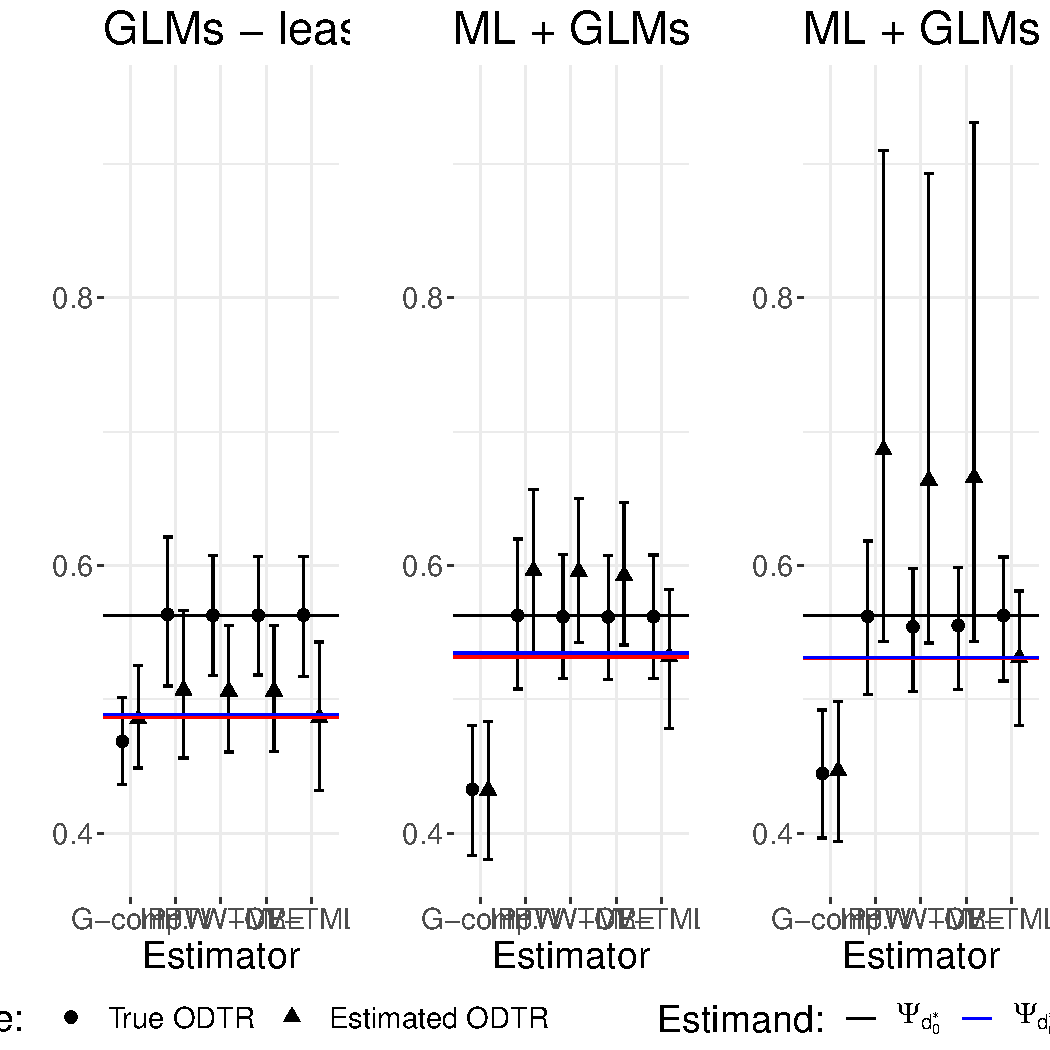
\includegraphics[width=\maxwidth]{figure/unnamed-chunk-1-1} 
\begin{kframe}\begin{verbatim}
## pdf 
##   2
\end{verbatim}
\end{kframe}
\end{knitrout}

\begin{knitrout}
\definecolor{shadecolor}{rgb}{0.969, 0.969, 0.969}\color{fgcolor}\begin{kframe}
\begin{alltt}
\hlkwd{make_table_EYdopt}\hlstd{(}\hlkwc{EYdopt} \hlstd{= EYdoptbin_glms,} \hlkwc{truevalues} \hlstd{= DGP_bin_complex_true_values)}
\end{alltt}
\begin{verbatim}
##                     Bias Variance    MSE Coverage        Estimator
## unadj            -0.0562    7e-04 0.0038    31.8%            unadj
## gcomp            -0.0773    4e-04 0.0064        -            gcomp
## IPTW             -0.0558    8e-04 0.0039      45%             IPTW
## IPTW_DR          -0.0565    6e-04 0.0038    30.1%          IPTW_DR
## TMLE             -0.0565    6e-04 0.0038    29.8%             TMLE
## LTMLE                 NA       NA     NA        -            LTMLE
## CV.TMLE          -0.0764    9e-04 0.0067    14.7%          CV.TMLE
## unadj_dopt0       0.0003    5e-04 0.0005    93.3%      unadj_dopt0
## gcomp_dopt0      -0.0940    3e-04 0.0091        -      gcomp_dopt0
## IPTW_dopt0        0.0009    8e-04 0.0008    95.3%       IPTW_dopt0
## IPTW_DR_dopt0     0.0001    5e-04 0.0005    93.7%    IPTW_DR_dopt0
## TMLE_dopt0        0.0002    5e-04 0.0005    93.7%       TMLE_dopt0
## LTMLE_dopt0           NA       NA     NA        -      LTMLE_dopt0
## CV.TMLE_dopt0     0.0004    5e-04 0.0005    93.7%    CV.TMLE_dopt0
## unadj_sampspec    0.0179    7e-04 0.0007    90.7%   unadj_sampspec
## gcomp_sampspec   -0.0033    4e-04 0.0006        -   gcomp_sampspec
## IPTW_sampspec     0.0183    8e-04 0.0009    94.3%    IPTW_sampspec
## IPTW_DR_sampspec  0.0175    6e-04 0.0007    90.6% IPTW_DR_sampspec
## LTMLE_sampspec        NA       NA     NA        -   LTMLE_sampspec
## TMLE_sampspec     0.0175    6e-04 0.0007    90.7%    TMLE_sampspec
## CV.TMLE_sampspec -0.0002    9e-04 0.0005    94.3% CV.TMLE_sampspec
\end{verbatim}
\begin{alltt}
\hlkwd{make_table_EYdopt}\hlstd{(}\hlkwc{EYdopt} \hlstd{= EYdoptbin_MLnotaggglms,} \hlkwc{truevalues} \hlstd{= DGP_bin_complex_true_values)}
\end{alltt}
\begin{verbatim}
##                     Bias Variance    MSE Coverage        Estimator
## unadj             0.0245    7e-04 0.0013    75.1%            unadj
## gcomp            -0.1306    7e-04 0.0178        -            gcomp
## IPTW              0.0334    1e-03 0.0021    76.1%             IPTW
## IPTW_DR           0.0327    8e-04 0.0019    66.5%          IPTW_DR
## TMLE              0.0298    8e-04 0.0016    71.3%             TMLE
## LTMLE                 NA       NA     NA        -            LTMLE
## CV.TMLE          -0.0308    7e-04 0.0017      69%          CV.TMLE
## unadj_dopt0      -0.0007    5e-04 0.0005    94.7%      unadj_dopt0
## gcomp_dopt0      -0.1298    6e-04 0.0175        -      gcomp_dopt0
## IPTW_dopt0        0.0002    8e-04 0.0008    94.7%       IPTW_dopt0
## IPTW_DR_dopt0    -0.0009    6e-04 0.0006      94%    IPTW_DR_dopt0
## TMLE_dopt0       -0.0011    5e-04 0.0005    93.6%       TMLE_dopt0
## LTMLE_dopt0           NA       NA     NA        -      LTMLE_dopt0
## CV.TMLE_dopt0    -0.0009    5e-04 0.0005    93.2%    CV.TMLE_dopt0
## unadj_sampspec    0.0524    7e-04 0.0033    36.2%   unadj_sampspec
## gcomp_sampspec   -0.1027    7e-04 0.0114        -   gcomp_sampspec
## IPTW_sampspec     0.0614    1e-03 0.0046    43.8%    IPTW_sampspec
## IPTW_DR_sampspec  0.0607    8e-04 0.0044    28.9% IPTW_DR_sampspec
## LTMLE_sampspec        NA       NA     NA        -   LTMLE_sampspec
## TMLE_sampspec     0.0578    8e-04 0.0040    30.4%    TMLE_sampspec
## CV.TMLE_sampspec  0.0002    7e-04 0.0005      94% CV.TMLE_sampspec
\end{verbatim}
\begin{alltt}
\hlkwd{make_table_EYdopt}\hlstd{(}\hlkwc{EYdopt} \hlstd{= EYdoptbin_MLaggglms,} \hlkwc{truevalues} \hlstd{= DGP_bin_complex_true_values)}
\end{alltt}
\begin{verbatim}
##                     Bias Variance    MSE Coverage        Estimator
## unadj             0.1138   0.0113 0.0243    29.9%            unadj
## gcomp            -0.1161   0.0007 0.0142        -            gcomp
## IPTW              0.1236   0.0109 0.0262      31%             IPTW
## IPTW_DR           0.1010   0.0092 0.0194      33%          IPTW_DR
## TMLE              0.1031   0.0108 0.0214    33.6%             TMLE
## LTMLE                 NA       NA     NA        -            LTMLE
## CV.TMLE          -0.0316   0.0007 0.0017    68.6%          CV.TMLE
## unadj_dopt0      -0.0001   0.0005 0.0005    93.7%      unadj_dopt0
## gcomp_dopt0      -0.1180   0.0006 0.0146        -      gcomp_dopt0
## IPTW_dopt0       -0.0006   0.0009 0.0009      94%       IPTW_dopt0
## IPTW_DR_dopt0    -0.0084   0.0005 0.0006    90.1%    IPTW_DR_dopt0
## TMLE_dopt0       -0.0075   0.0005 0.0006    90.6%       TMLE_dopt0
## LTMLE_dopt0           NA       NA     NA        -      LTMLE_dopt0
## CV.TMLE_dopt0    -0.0001   0.0005 0.0005    93.6%    CV.TMLE_dopt0
## unadj_sampspec    0.1453   0.0113 0.0342    12.3%   unadj_sampspec
## gcomp_sampspec   -0.0846   0.0007 0.0081        -   gcomp_sampspec
## IPTW_sampspec     0.1551   0.0109 0.0366    16.3%    IPTW_sampspec
## IPTW_DR_sampspec  0.1325   0.0092 0.0283    15.8% IPTW_DR_sampspec
## LTMLE_sampspec        NA       NA     NA        -   LTMLE_sampspec
## TMLE_sampspec     0.1346   0.0108 0.0307    15.7%    TMLE_sampspec
## CV.TMLE_sampspec  0.0001   0.0007 0.0005    94.8% CV.TMLE_sampspec
\end{verbatim}
\end{kframe}
\end{knitrout}

\begin{knitrout}
\definecolor{shadecolor}{rgb}{0.969, 0.969, 0.969}\color{fgcolor}\begin{kframe}
\begin{verbatim}
##                        Comparison                  Library Estimator    Bias
## unadj_sampspec    EnYdn for E0Ydn                     GLMs    Unadj.  0.0179
## gcomp_sampspec    EnYdn for E0Ydn                     GLMs   G-comp. -0.0033
## IPTW_sampspec     EnYdn for E0Ydn                     GLMs      IPTW  0.0183
## IPTW_DR_sampspec  EnYdn for E0Ydn                     GLMs   IPTW-DR  0.0175
## TMLE_sampspec     EnYdn for E0Ydn                     GLMs      TMLE  0.0175
## CV.TMLE_sampspec  EnYdn for E0Ydn                     GLMs   CV-TMLE -0.0002
## unadj_sampspec1   EnYdn for E0Ydn ML + GLMs not aggressive    Unadj.  0.0524
## gcomp_sampspec1   EnYdn for E0Ydn ML + GLMs not aggressive   G-comp. -0.1027
## IPTW_sampspec1    EnYdn for E0Ydn ML + GLMs not aggressive      IPTW  0.0614
## IPTW_DR_sampspec1 EnYdn for E0Ydn ML + GLMs not aggressive   IPTW-DR  0.0607
## TMLE_sampspec1    EnYdn for E0Ydn ML + GLMs not aggressive      TMLE  0.0578
## CV.TMLE_sampspec1 EnYdn for E0Ydn ML + GLMs not aggressive   CV-TMLE  0.0002
## unadj_sampspec2   EnYdn for E0Ydn     ML + GLMs aggressive    Unadj.  0.1453
## gcomp_sampspec2   EnYdn for E0Ydn     ML + GLMs aggressive   G-comp. -0.0846
## IPTW_sampspec2    EnYdn for E0Ydn     ML + GLMs aggressive      IPTW  0.1551
## IPTW_DR_sampspec2 EnYdn for E0Ydn     ML + GLMs aggressive   IPTW-DR  0.1325
## TMLE_sampspec2    EnYdn for E0Ydn     ML + GLMs aggressive      TMLE  0.1346
## CV.TMLE_sampspec2 EnYdn for E0Ydn     ML + GLMs aggressive   CV-TMLE  0.0001
##                   Variance    MSE Coverage
## unadj_sampspec      0.0007 0.0007    90.7%
## gcomp_sampspec      0.0004 0.0006        -
## IPTW_sampspec       0.0008 0.0009    94.3%
## IPTW_DR_sampspec    0.0006 0.0007    90.6%
## TMLE_sampspec       0.0006 0.0007    90.7%
## CV.TMLE_sampspec    0.0009 0.0005    94.3%
## unadj_sampspec1     0.0007 0.0033    36.2%
## gcomp_sampspec1     0.0007 0.0114        -
## IPTW_sampspec1      0.0010 0.0046    43.8%
## IPTW_DR_sampspec1   0.0008 0.0044    28.9%
## TMLE_sampspec1      0.0008 0.0040    30.4%
## CV.TMLE_sampspec1   0.0007 0.0005      94%
## unadj_sampspec2     0.0113 0.0342    12.3%
## gcomp_sampspec2     0.0007 0.0081        -
## IPTW_sampspec2      0.0109 0.0366    16.3%
## IPTW_DR_sampspec2   0.0092 0.0283    15.8%
## TMLE_sampspec2      0.0108 0.0307    15.7%
## CV.TMLE_sampspec2   0.0007 0.0005    94.8%
##                     Comparison                  Library Estimator    Bias
## unadj_dopt0    EnYd0 for E0Yd0                     GLMs    Unadj.  0.0003
## gcomp_dopt0    EnYd0 for E0Yd0                     GLMs   G-comp. -0.0940
## IPTW_dopt0     EnYd0 for E0Yd0                     GLMs      IPTW  0.0009
## IPTW_DR_dopt0  EnYd0 for E0Yd0                     GLMs   IPTW-DR  0.0001
## TMLE_dopt0     EnYd0 for E0Yd0                     GLMs      TMLE  0.0002
## CV.TMLE_dopt0  EnYd0 for E0Yd0                     GLMs   CV-TMLE  0.0004
## unadj_dopt01   EnYd0 for E0Yd0 ML + GLMs not aggressive    Unadj. -0.0007
## gcomp_dopt01   EnYd0 for E0Yd0 ML + GLMs not aggressive   G-comp. -0.1298
## IPTW_dopt01    EnYd0 for E0Yd0 ML + GLMs not aggressive      IPTW  0.0002
## IPTW_DR_dopt01 EnYd0 for E0Yd0 ML + GLMs not aggressive   IPTW-DR -0.0009
## TMLE_dopt01    EnYd0 for E0Yd0 ML + GLMs not aggressive      TMLE -0.0011
## CV.TMLE_dopt01 EnYd0 for E0Yd0 ML + GLMs not aggressive   CV-TMLE -0.0009
## unadj_dopt02   EnYd0 for E0Yd0     ML + GLMs aggressive    Unadj. -0.0001
## gcomp_dopt02   EnYd0 for E0Yd0     ML + GLMs aggressive   G-comp. -0.1180
## IPTW_dopt02    EnYd0 for E0Yd0     ML + GLMs aggressive      IPTW -0.0006
## IPTW_DR_dopt02 EnYd0 for E0Yd0     ML + GLMs aggressive   IPTW-DR -0.0084
## TMLE_dopt02    EnYd0 for E0Yd0     ML + GLMs aggressive      TMLE -0.0075
## CV.TMLE_dopt02 EnYd0 for E0Yd0     ML + GLMs aggressive   CV-TMLE -0.0001
##                Variance    MSE Coverage
## unadj_dopt0       5e-04 0.0005    93.3%
## gcomp_dopt0       3e-04 0.0091        -
## IPTW_dopt0        8e-04 0.0008    95.3%
## IPTW_DR_dopt0     5e-04 0.0005    93.7%
## TMLE_dopt0        5e-04 0.0005    93.7%
## CV.TMLE_dopt0     5e-04 0.0005    93.7%
## unadj_dopt01      5e-04 0.0005    94.7%
## gcomp_dopt01      6e-04 0.0175        -
## IPTW_dopt01       8e-04 0.0008    94.7%
## IPTW_DR_dopt01    6e-04 0.0006      94%
## TMLE_dopt01       5e-04 0.0005    93.6%
## CV.TMLE_dopt01    5e-04 0.0005    93.2%
## unadj_dopt02      5e-04 0.0005    93.7%
## gcomp_dopt02      6e-04 0.0146        -
## IPTW_dopt02       9e-04 0.0009      94%
## IPTW_DR_dopt02    5e-04 0.0006    90.1%
## TMLE_dopt02       5e-04 0.0006    90.6%
## CV.TMLE_dopt02    5e-04 0.0005    93.6%
##               Comparison                  Library Estimator    Bias Variance
## unadj    EnYdn for E0Yd0                     GLMs    Unadj. -0.0562   0.0007
## gcomp    EnYdn for E0Yd0                     GLMs   G-comp. -0.0773   0.0004
## IPTW     EnYdn for E0Yd0                     GLMs      IPTW -0.0558   0.0008
## IPTW_DR  EnYdn for E0Yd0                     GLMs   IPTW-DR -0.0565   0.0006
## TMLE     EnYdn for E0Yd0                     GLMs      TMLE -0.0565   0.0006
## CV.TMLE  EnYdn for E0Yd0                     GLMs   CV-TMLE -0.0764   0.0009
## unadj1   EnYdn for E0Yd0 ML + GLMs not aggressive    Unadj.  0.0245   0.0007
## gcomp1   EnYdn for E0Yd0 ML + GLMs not aggressive   G-comp. -0.1306   0.0007
## IPTW1    EnYdn for E0Yd0 ML + GLMs not aggressive      IPTW  0.0334   0.0010
## IPTW_DR1 EnYdn for E0Yd0 ML + GLMs not aggressive   IPTW-DR  0.0327   0.0008
## TMLE1    EnYdn for E0Yd0 ML + GLMs not aggressive      TMLE  0.0298   0.0008
## CV.TMLE1 EnYdn for E0Yd0 ML + GLMs not aggressive   CV-TMLE -0.0308   0.0007
## unadj2   EnYdn for E0Yd0     ML + GLMs aggressive    Unadj.  0.1138   0.0113
## gcomp2   EnYdn for E0Yd0     ML + GLMs aggressive   G-comp. -0.1161   0.0007
## IPTW2    EnYdn for E0Yd0     ML + GLMs aggressive      IPTW  0.1236   0.0109
## IPTW_DR2 EnYdn for E0Yd0     ML + GLMs aggressive   IPTW-DR  0.1010   0.0092
## TMLE2    EnYdn for E0Yd0     ML + GLMs aggressive      TMLE  0.1031   0.0108
## CV.TMLE2 EnYdn for E0Yd0     ML + GLMs aggressive   CV-TMLE -0.0316   0.0007
##             MSE Coverage
## unadj    0.0038    31.8%
## gcomp    0.0064        -
## IPTW     0.0039      45%
## IPTW_DR  0.0038    30.1%
## TMLE     0.0038    29.8%
## CV.TMLE  0.0067    14.7%
## unadj1   0.0013    75.1%
## gcomp1   0.0178        -
## IPTW1    0.0021    76.1%
## IPTW_DR1 0.0019    66.5%
## TMLE1    0.0016    71.3%
## CV.TMLE1 0.0017      69%
## unadj2   0.0243    29.9%
## gcomp2   0.0142        -
## IPTW2    0.0262      31%
## IPTW_DR2 0.0194      33%
## TMLE2    0.0214    33.6%
## CV.TMLE2 0.0017    68.6%
\end{verbatim}
\end{kframe}
\end{knitrout}

\section{Summary of Results Above}

\begin{itemize}
    \item \underline{\textbf{$E_n[Y_{d_0}]$ to estimate $E_0[Y_{d_0}]$}}: these results speak to performance of estimators of $E_0[Y_{d}]$ for some given $d$ (i.e., not about how well we estimate the rule, but about how well we estimate the performance of a given rule, which here it happens to be $d_0$). Estimator results:
    \begin{itemize}
        \item g-comp: biased
        \begin{itemize}
            \item Note: this differs from estimation of, e.g., $E[Y_1]$ in RCT (or using any treatment rule that isn't a function of covariates), where g-comp using a misspecified glm is a TMLE, and therefore unbiased
        \end{itemize}
        \item IPTW: less efficient (more variability), including less efficient than unadjusted
        \begin{itemize}
            \item Note: this again differs from estimation of, e.g., $E[Y_1]$ in RCT, where IPTW using estimated weights we gain efficiency
        \end{itemize}
        \item IPTW-DR and TMLE: unbiased, EXCEPT if $Q$ estimated aggressively, then bias enough for coverage to drop to $\sim 90\%$
        \begin{itemize}
            \item Small variance gain compared to unadjusted (though suspect this gain would be bigger if covariates were more predictive of outcome?)
        \end{itemize}
\item CV-TMLE: unbiased (even with more aggressive library for $Q$)
\item Unadjusted: unbiased
\begin{itemize}
    \item Small variance price vs the DR estimators, but without risk of bias due to overfitting $Q$
    \item Very little difference compared to CV-TMLE
\end{itemize}
    \end{itemize}
    \item \underline{\textbf{$E_n[Y_{d_n}]$ to estimate $E_0[Y_{d_0}]$}}: these results speak to not only how good of a job we do evaluating the rule (i.e., as above), but also how well we estimate the rule
    \begin{itemize}
        \item None do well. This is all due to fall off in estimating $d_0$, ie $d_n$ not converging to $d_0$ fast enough.
        \begin{itemize}
            \item See ODTR paper just submitted- how to do a better job on $d_0$ (including at finite sample sizes, even if cant get all the way there, how to get closer)
        \end{itemize}
    \end{itemize}
    \item \textbf{\underline{$E_n[Y_{d_n}]$ to estimate $E_0[Y_{d_n}]$}}: these results are of interest if going after a data-adaptive target parameter
    \begin{itemize}
        \item Note: the estimators are targeting different data adaptive parameters. Data-adaptive parameter here for CV-TMLE is the average of the folds, for the others, it is the $d_n$ learned on the whole sample
        \begin{itemize}
            \item However, here they are pretty similar
        \end{itemize}
        \item There is a real price in bias paid by not using sample splitting to evaluate performance
        \begin{itemize}
            \item For all of the other estimators besides CV-TMLE, will overestimate how well the estimated rule does
            \item As the library used to estimate Q gets more aggressive:
            \begin{itemize}
                \item The estimated rule gets closer to the true rule
                \item The price paid (in terms of bias) by not using CV-TMLE increases
            \end{itemize}
        \end{itemize}
    \end{itemize}
\end{itemize}


\noindent Big picture summary:
\begin{itemize}
    \item For large sample sizes, small price and many benefits to using CV-TMLE with aggressive library to estimate $E_0[Y_{d_0}]$ and $E_0[Y_{d_n}]$
    \begin{itemize}
        \item But, is this true if truth is simple? If sample size is small, worry is in that case pay a price. We want a method that as sample size increases, goes towards the more complex; when sample size limited, data can't support, will go towards simple (CI-based ODTR might help here)
    \end{itemize}
\end{itemize}


\end{document}
